\documentclass[a4paper,10pt]{article}
\usepackage[brazilian]{babel}
\usepackage[left=2.5cm,right=2.5cm,top=3cm,bottom=2.5cm]{geometry}
\usepackage{mathtools}
\usepackage{amsthm}
\usepackage{amsmath}
%\usepackage{nccmath}
\usepackage{amssymb}
\usepackage{amsfonts}
\usepackage{physics}
%\usepackage{dsfont}
%\usepackage{mathrsfs}

\usepackage{titling}
\usepackage{indentfirst}

\usepackage{bm}
\usepackage[dvipsnames]{xcolor}
\usepackage{cancel}

\usepackage{xurl}
\usepackage[colorlinks=true]{hyperref}

\usepackage{float}
\usepackage{graphicx}
%\usepackage{tikz}
\usepackage{caption}
\usepackage{subcaption}

%%%%%%%%%%%%%%%%%%%%%%%%%%%%%%%%%%%%%%%%%%%%%%%%%%%

\newcommand{\eps}{\epsilon}
\newcommand{\vphi}{\varphi}
\newcommand{\cte}{\text{cte}}

\newcommand{\N}{\mathbb{N}}
\newcommand{\Z}{\mathbb{Z}}
\newcommand{\Q}{\mathbb{Q}}
\newcommand{\R}{\vb{R}}
\newcommand{\C}{\mathbb{C}}
\renewcommand{\S}{\hat{S}}
%\renewcommand{\H}{\s{H}}

\renewcommand{\a}{\vb{a}}
\newcommand{\nn}{\hat{n}}
\renewcommand{\d}{\dagger}
\newcommand{\up}{\uparrow}
\newcommand{\down}{\downarrow}

\newcommand{\0}{\vb{0}}
%\newcommand{\1}{\mathds{1}}
\newcommand{\E}{\vb{E}}
\newcommand{\B}{\vb{B}}
\renewcommand{\v}{\vb{v}}
\renewcommand{\r}{\vb{r}}
\renewcommand{\k}{\vb{k}}
\newcommand{\p}{\vb{p}}
\newcommand{\q}{\vb{q}}
\newcommand{\F}{\vb{F}}

\newcommand{\s}{\sigma}
%\newcommand{\prodint}[2]{\left\langle #1 , #2 \right\rangle}
\newcommand{\cc}[1]{\overline{#1}}
\newcommand{\Eval}[3]{\eval{\left( #1 \right)}_{#2}^{#3}}

\newcommand{\unit}[1]{\; \mathrm{#1}}

\newcommand{\n}{\medskip}
\newcommand{\e}{\quad \mathrm{e} \quad}
\newcommand{\ou}{\quad \mathrm{ou} \quad}
\newcommand{\virg}{\, , \;}
\newcommand{\ptodo}{\forall \,}
\renewcommand{\implies}{\; \Rightarrow \;}
%\newcommand{\eqname}[1]{\tag*{#1}} % Tag equation with name

\setlength{\droptitle}{-7em}

\theoremstyle{plain}
\newtheorem{theorem}{Teorema}[section]
%\newtheorem{defi}[theorem]{Definição}
\newtheorem{lemma}[theorem]{Lema}
%\newtheorem{corol}[theorem]{Corolário}
%\newtheorem{prop}[theorem]{Proposição}
%\newtheorem{example}{Exemplo}
%
%\newtheorem{inneraxiom}{Axioma}
%\newenvironment{axioma}[1]
%  {\renewcommand\theinneraxiom{#1}\inneraxiom}
%  {\endinneraxiom}
%
%\newtheorem{innerpostulado}{Postulado}
%\newenvironment{postulado}[1]
%  {\renewcommand\theinnerpostulado{#1}\innerpostulado}
%  {\endinnerpostulado}
%
%\newtheorem{innerexercise}{Exercício}
%\newenvironment{exercise}[1]
%  {\renewcommand\theinnerexercise{#1}\innerexercise}
%  {\endinnerexercise}
%
%\newtheorem{innerthm}{Teorema}
%\newenvironment{teorema}[1]
%  {\renewcommand\theinnerthm{#1}\innerthm}
%  {\endinnerthm}
%
\newtheorem{innerlema}{Lema}
\newenvironment{lema}[1]
  {\renewcommand\theinnerlema{#1}\innerlema}
  {\endinnerlema}
%
%\theoremstyle{remark}
%\newtheorem*{hint}{Dica}
%\newtheorem*{notation}{Notação}
%\newtheorem*{obs}{Observação}


\title{\Huge{\textbf{Lista 4 - Matéria Condensada 2}}}
\author{Mateus Marques}

\begin{document}

\maketitle

\section{Fórmula de Drude revisitada}

Neste caso, o campo elétrico $\E(t) = \E(\omega) e^{-i\omega t}$ é estático (e o magnético zero $\vb{H}=\0$), porém dependente do tempo. Dessa forma, a função distribuição $f(\k, t)$ depende apenas do momento $\k$ e do tempo $t$. A equação de Boltzmann dentro da aproximação do tempo de relaxação então fica
$$
\qty[\pdv{t} + \dot{\k} \vdot \grad_{\k}] f(\k, t) =
-\frac{1}{\tau} \qty[f(\k,t) - f_0(\k)],
$$
onde $f_0(\k) = \frac{1}{\exp[\beta(\eps_n(\k)-\mu)] + 1}$ é a distribuição de Fermi-Dirac. Da equação semiclássica
$$
\hbar \dot{\k} = -e \qty[\E + \frac{1}{c} \v_n(\k) \cp \vb{H}],
$$
temos que $\dot{\k} = - \frac{e \E(t)}{\hbar} = -\frac{e \E(\omega)}{\hbar} e^{-i\omega t}$ (colocarei $\hbar=1$). Definindo $\delta f(\k,t) = f(\k,t) - f_0(\k)$ e utilizando a aproximação linear que $\delta f(\k,t) \propto \E(t) = \E(\omega) e^{-i\omega t}$, temos $\pdv{t} \delta f(\k,t) = - i\omega \delta f(\k,t)$. Portanto:
$$
\pdv{t}\delta f(\k,t) + \frac{1}{\tau} \delta f(\k, t) =  - \dot{\k} \vdot \grad_{\k}  [f_0(\k) + \delta f(\k, t) ] \implies
$$
$$
\delta f(\k,t) = \frac{e \tau}{1-i\omega \tau} \, \E(t) \vdot \grad_{\k}  [ f_0(\k) + \delta f(\k, t) ].
$$
Note que a equação acima é um equação de ponto fixo para $\delta f(\k,t)$. Mas como nos basta a aproximação linear onde $\delta f(\k,t)$ é proporcional a $\E(t)$, ficamos com
$$
\delta f(\k,t) \simeq \frac{e \tau}{1-i\omega \tau} \, \E(t) \vdot \grad_{\k}  f_0(\k).
$$
Utilizando a expressão para a densidade de corrente em duas dimensões
$$
\vb{j}_n = -e \int \frac{\dd[2]{\k}}{(2\pi)^2} \v_n(\k) f(\k),
$$
temos
$$
\vb{j}_n = -e \int \frac{\dd[2]{\k}}{(2\pi)^2} \v_n(\k)
\qty{ \cancelto{0}{f_0(\k)} +
\frac{\tau[\eps_n(\k)]}{1-i\omega \tau[\eps_n(\k)]} e\E \vdot \grad_{\k} f_0(\k)} =
$$
$$
= e^2 \int \frac{\dd[2]{\k}}{(2\pi)^2} \v_n(\k)
\frac{\tau[\eps_n(\k)]}{1-i\omega \tau[\eps_n(\k)]} \qty(-\pdv{f_0(\k)}{\eps(\k)}) \, \E \vdot
\cancelto{\v_n(\k)}{\grad_k \eps_n(\k)} =
$$
$$
= e^2 \int \frac{\dd[2]{\k}}{(2\pi)^2} \v_n(\k) ( \v_n(\k) \vdot \E )
\frac{\tau[\eps_n(\k)]\qty(-\partial f_0 / \partial \eps)_{\eps = \eps_n(\k)}}{1-i\omega \tau[\eps_n(\k)]}.
$$
Como definimos $j^{\mu} = \sum_{\nu} \s^{\mu\nu} E^{\nu}$, vemos facilmente que
$$
\sigma^{\mu\nu}_{(n)}(\omega) = e^2 \int \frac{\dd[2]{\k}}{(2\pi)^2}
\frac{v_n^{\mu}(\k) v_n^{\nu}(\k) \, \tau[\eps_n(\k)] \, \qty(-\partial f_0 / \partial \eps)_{\eps = \eps_n(\k)}}
{1-i\omega \tau[\eps_n(\k)]}.
$$

Supondo que $\tau[\eps_n(\k)]$ tenha um valor bem definido $\tau_F$ na superfície de Fermi, no limite $T \to 0$ temos $\qty(-\partial f_0 / \partial \eps)_{\eps = \eps_n(\k)} \to \delta(\eps_n(\k) - E_F)$ e portanto
$$
\sigma(\omega) = e^2 \int \frac{\dd[2]{\k}}{(2\pi)^2}
\frac{\v(\k) \v(\k) \, \tau[\eps_n(\k)] \, \delta(\eps_n(\k) - E_F)}
{1-i\omega \tau[\eps_n(\k)]} =
e^2 \frac{v_F^2 \, \tau_F }{1-i\omega \tau_F}
\int \frac{\dd[2]{\k}}{(2\pi)^2} \, \delta(\eps_n(\k) - E_F) \implies
$$
$$
\s(\omega) = e^2 \frac{v_F^2 \, \tau_F }{1-i\omega \tau_F} \, \rho(E_F)
$$

INCLUIR ISOTROPIA (DIVIDIR POR DIMENSÕES), CORRIGIR $\s$ e EXPLICAR o fator de $n$.


\pagebreak

\section{Condutividade eletrônica}

Por equipartição da energia (isotropia) temos na superfície de Fermi $3v^2 = v_F^2$. Para baixas temperaturas $T \to 0$ temos então
$$
\s = \frac{2e^2 v_F^2 \tau_F}{3} \int \frac{\dd[3]{\k}}{(2\pi)^3}
\qty(-\pdv{f}{\eps})_{\eps=\eps(\k)} =
\frac{2e^2 v_F^2 \tau_F}{3} \int \frac{\dd[3]{\k}}{(2\pi)^3}
\int \dd{\eps} \delta(\eps - \eps(\k)) \qty(-\pdv{f}{\eps}) =
$$
$$
\s = \frac{2e^2 v_F^2 \tau_F}{3} \int \dd{\eps} \rho(\eps) \qty(-\pdv{f}{\eps}).
$$

Integrando por partes:
$$
\int \dd{\eps} \rho(\eps) \qty(-\pdv{f}{\eps}) =
\int \dd{\eps} f(\eps) \dv{\rho}{\eps}.
$$

A partir de agora assumiremos $E_F$, $T_F = D = k_B = 1$.

\begin{itemize}
\item (a) Metal: $\rho(\eps) = \frac{4}{\pi} \sqrt{1-\eps^2}$. Para $T \to 0$ podemos usar a expansão de Sommerfeld
$$
\int_{-\infty}^{\infty} \dd{\eps} f(\eps) G(\eps) \simeq
\int_{-\infty}^{\mu} G(\eps) + \frac{\pi^2}{6} T^2 \eval{\dv{G}{\eps}}_{\eps=\mu}.
$$
Colocando $G(\eps) = \dd{\rho}/\dd{\eps}$ temos
$$
\s = \frac{2e^2 v_F^2 \tau_F}{3}
\int_{-\infty}^{\infty} \dd{\eps} f(\eps) \dv{\rho}{\eps} =
\frac{2e^2 v_F^2 \tau_F}{3}
\qty{\rho(E_F) + \frac{\pi^2}{6} T^2 \eval{\dv[2]{\rho}{\eps}}_{\eps=E_F}}.
$$
Assim, da expressão $\s = \s_0 - A T^2$, reconhecemos
$$
\s_0 = \frac{2e^2 v_F^2 \tau_F}{3} \rho(E_F) \e
A = -\frac{2e^2v_F^2\tau_F}{3} \frac{\pi^2}{6} \eval{\dv[2]{\rho}{\eps}}_{\eps=E_F}.
$$

\textbf{ESBOÇO $\rho(\eps)$ e $\s(T)$. VERIFICAR QUE $\int\rho=2$}. COMENTAR O GRÁFICO.

\item (b) Semimetal: $\rho(\eps)=2\abs{\eps}$.

\item (c) Semicondutor: $\rho(\eps) = \frac{\eps}{\sqrt{\eps^2-\Delta^2}}$, $\Delta < \eps < 1$. Como obter $\Delta$ a partir somente do $\s(T)$?

Observação: basicamente temos $T \to 0$. Então em baixas energias temos que cada sistema se comporta com o $\rho(\eps)$ da categoria. Ainda mais, podemos sempre setar $E_F = 0$.

\begin{figure}[H]
\centering
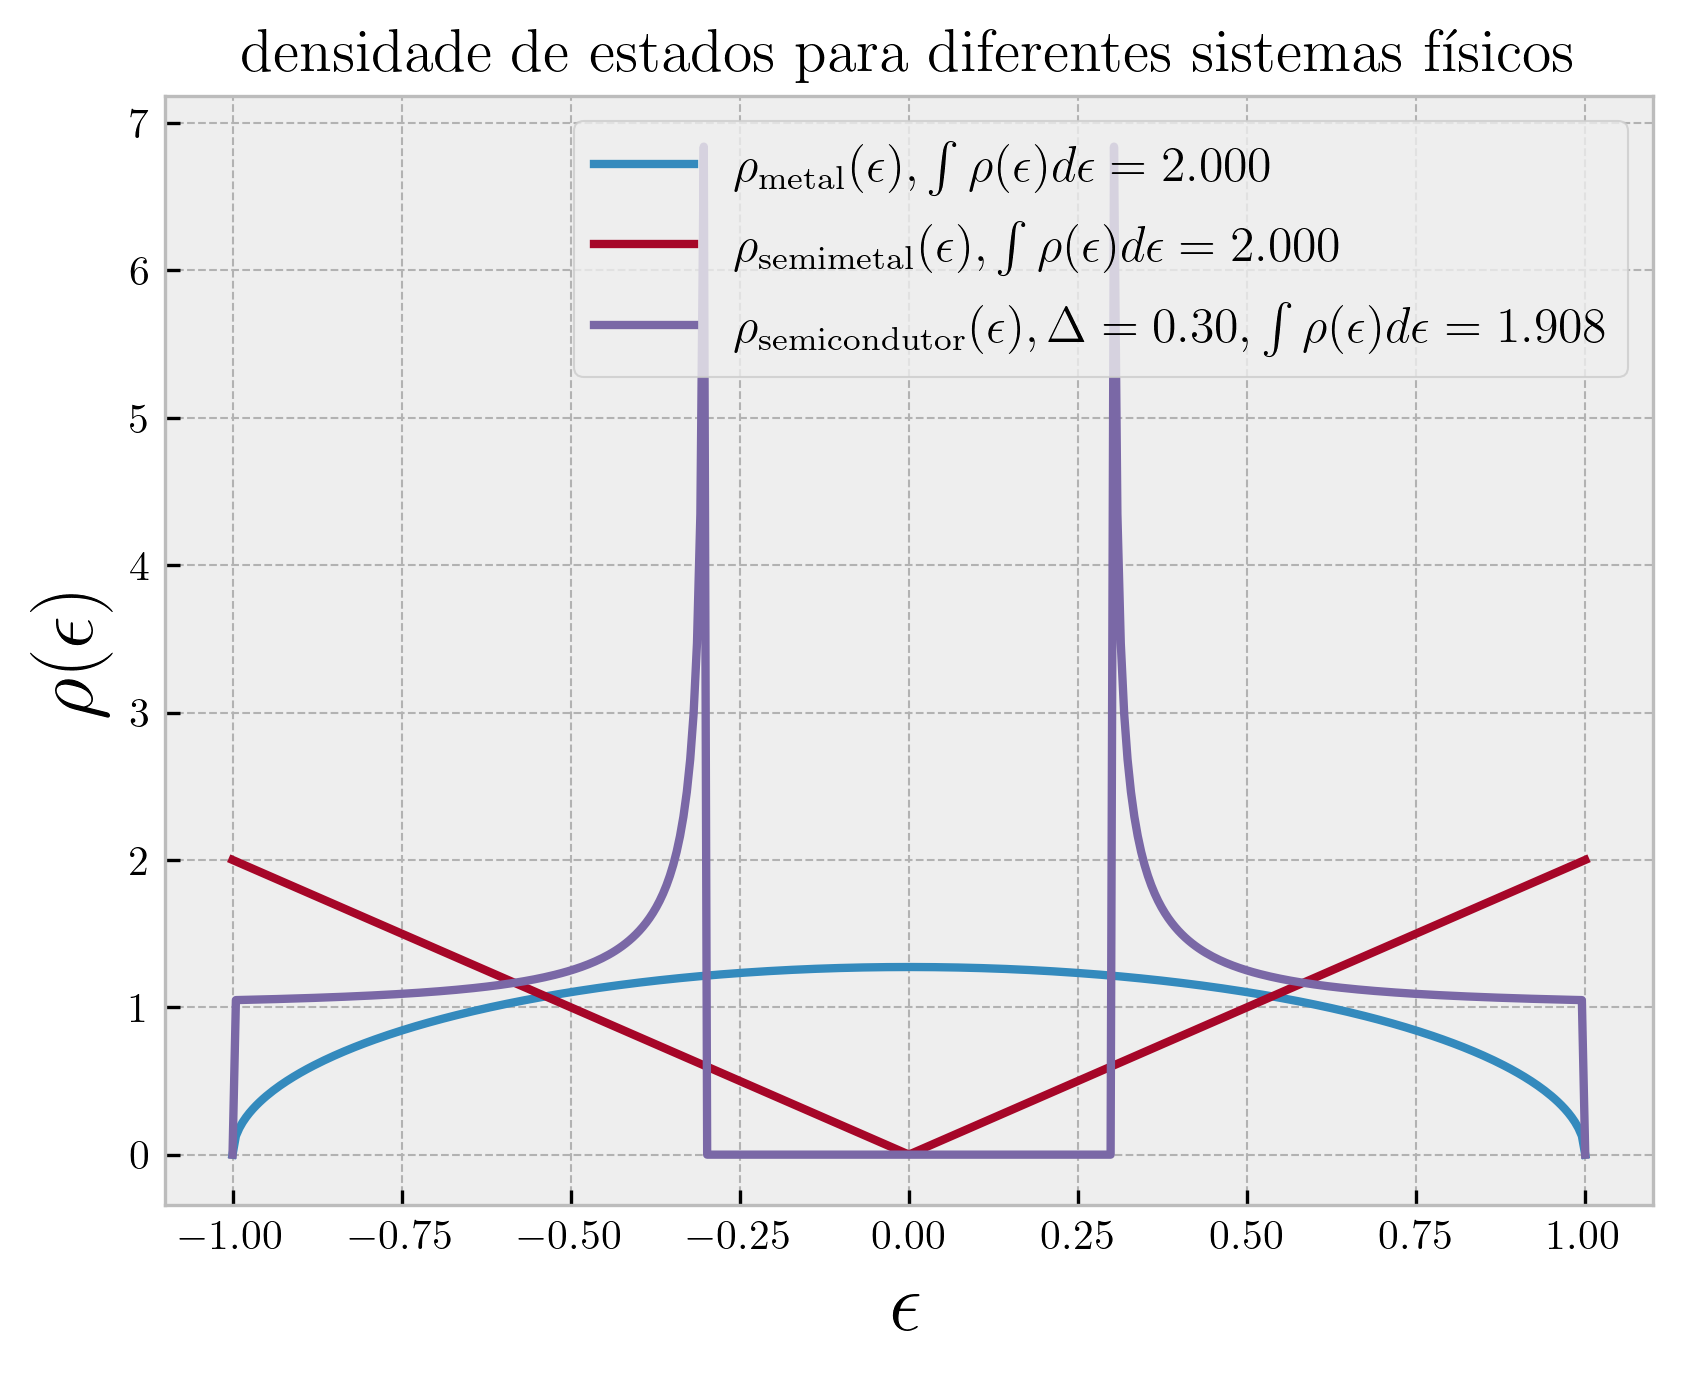
\includegraphics[width=0.6\textwidth]{fig/dos-systems.png}
\caption{Densidade de estados para os sistemas metal, semimetal e semicondutor.}
\label{fig:dos-systems}
\end{figure}
Note que obtivemos $1.999$ ao invés de $2$ para o caso semicondutor. Para fazer esse cálculo, utilizei a função \texttt{scipy.integrate.quad} e explicitei que os pontos $\pm\Delta$ são pontos de divergência. Mesmo assim a integral não resultou em $2$ exatamente.

Percebi que na verdade temos $\int \frac{x}{\sqrt{x^2-\Delta^2}} \dd{x} = \sqrt{x^2 - \Delta^2}$, de maneira que
$$
\int_{-1}^{-\Delta} \frac{\abs{\eps}}{\eps^2-\Delta^2} \dd{\eps} + \int_{\Delta}^{1} \frac{\eps}{\eps^2-\Delta^2} \dd{\eps} = 2 \sqrt{1-\Delta^2}.
$$
Assim, a integral não é exatamente $2$, a não ser que $\Delta = 0$.

\end{itemize}


\pagebreak

\section{Desordem e localização de Anderson}

\pagebreak

\section{Efeito Hall}

\pagebreak

\section{Número de Chern para um modelo de duas bandas}

\pagebreak

\section{Condutividade Hall}


\pagebreak

\end{document}
